\chapter{Floating-point representations}
\label{ch:background}
Among the different methods to represent the set of real numbers in computers,
floating-point is a commonly adopted format.
This chapter discusses some fundamental definitions and basic notions on floating-point
and briefly describes the IEEE~754~\cite{ieee754_2008-ev} data format.
We based the content in this chapter on~\cite{Muller2018-zm}.

\section{Definitions and basic notions}
A floating-point format is defined with four integers:
\begin{itemize}
	\item A \textit{radix} (or \textit{Base}) $B \ge 2$;
	\item A \textit{precision} $p \ge 2$, which approximately represents the number of significant digits for the format;
	\item Two exponents, $e_{min}$ and $e_{max}$, bound the value range represented by the format. In practice, $e_{min} \le 0 \le e_{max}$.
\end{itemize}

A floating-point number in such a format is a number $x$ that can be represented by a pair $(M,e)$, such that
\begin{equation}
	x = M \cdot B^{e-p+1}
\end{equation}
where
\begin{itemize}
	\item $M$ is an integer such that $|M| \le B^{p}-1$. It is called the \textit{integral significand} of x;
	\item $e$ is an integer such that $e_{min} \le e \le e_{max}$. It is called the \textit{exponent} of x.
\end{itemize}

Another way to represent a number $x$ as a floating-point number is with a triple $(s, m, e)$, such that
\begin{equation}
	x = (-1)^{s} \cdot m \cdot B^{e}
\end{equation}
where
\begin{itemize}
	\item $e$ is the same as before;
	\item $m = |M| \cdot B^{1-p}$ is the normal significand, commonly called mantissa;
	\item $s \in \{0, 1\}$ is the sign of $x$.
\end{itemize}

The representation of a number using a pair $(M, e)$ or $(s, m, e)$ is not unique.
The set of all such representations is called a \textit{cohort}.
\HL{
	However, it is desirable to have a unique floating-point representation for
	each number as it simplifies the expression of error bounds and the implementation
	of the data format.
	It can be achieved, for example, by always representing numbers using the minimum possible exponent.
	This is known as \textit{normalized representation}.
}

Floating points are often categorized into \textit{normal} and \textit{subnormal} (\textit{denormal}) numbers.
In radix 2, the first digit of the significand is 1 for normal numbers and 0 for subnormal ones.
\HL{
	This deterministic information enables an encoding strategy known as \textit{hidden bit convention} (described in Section~{\ref{sc:ieee754}}),
	which avoids storing the most significant bit while preserving the same precision.
	A number that is too large to be represented by a data format precision and exponent range is said to \textit{overflow}.
	Similarly, when a number is too close to zero and cannot be represented, it \textit{underflows}.
	The availability of subnormal numbers allows for \textit{gradual underflow},
	which would return an increasingly smaller subnormal value instead of zero in the case of an underflow.
	Mitigating the precision loss from underflows helps in implementing numerically stable code.
	Round-off error accumulation occurs when a series of arithmetic operations amplify
	an initially small error into a much larger one; the algorithm is said to be \textit{unstable}.
	Adding a large and small number requires shifting the mantissa bits of the
	smaller number to the right, resulting in a loss of precision for the smaller
	number; this is known as \textit{swamping}~{\cite{SwampCancel}}.
	Performing a subtraction of two approximately equal but distinct numbers
	will cancel the significant bit that both numbers have in common and leave
	out the difference from their least significant bits; this is known as \textit{catastrophic cancellation}~{\cite{SwampCancel}}.
	This issue can be problematic as the least significant bits of a number might
	be affected by rounding errors, thus carrying more errors into the subtraction.
}

A common way to define the error introduced by a floating-point arithmetic
operation is the \textit{unit in the last place (ulp)}.
\HL{Given a number x, represented as a floating-point,} $ulp(x)$ is defined as the distance between the two closest distinct
floating-point numbers $a$ and $b$, such that \HL{$a \le x \le b$} and $a \neq b$.
\HL{In other words, one ulp is equal to $B^{e-p+1}$, the smallest unit representable at a given exponent}.

\HL{
	When performing the arithmetic computation in a high-precision register, the
	intermediate result might be rounded to the precision of the CPU register
	and rounded again to the data format precision.
	This is known as \textit{double rounding}.
}
A function is \textit{correctly rounded} when it always rounds its results the 
same way as if it used infinite precision and range.
When a function cannot guarantee correct rounding and always rounds a number $y$
using one \textit{round-up} or \textit{round-down} function, it is said to be \textit{faithful}.
Correctly rounded functions are always faithful.
One must remember that even if a function is correctly rounded, there is
still a loss of information if the number cannot be represented exactly in the
floating-point format.

Some properties from real number arithmetic are lost with floating-point arithmetic, while others remain.
\HL{For example, arithmetic operations remain commutative with addition and multiplication when correctly rounded.}
However, associativity and distributivity no longer apply.
If not cautious about this, it can result in drastic errors.
	
						
\section{IEEE~754 Binary format}
\label{sc:ieee754}
Since the beginning of computers, there have been multiple proposed solutions to represent floating-point numbers.
This section limits our focus to the IEEE~754-2008 format, shortened to IEEE~754, as it is largely adopted in hardware.
The IEEE~754 format describes a standard for radix 2 and 10, Binary and Decimal, respectively.
We limit our scope to the Binary data type since Decimal is mainly used in financial applications, which are outside the scope of our research.
						
IEEE~754 defines three basic formats for Binary: 32, 64, and 128 bits.
It also defines a suggested format for 16 bits.
A precision size is defined in all those formats, and a range for the exponent values of $e_{min} = 1 - e_{max}$.
Table~\ref{table:IEEE754-binary-parameters} shows the precision and exponent parameters for each format. 
						
\begin{table}[h]
	\centering
	\begin{tabular}{|c|r|r|r|r|}
		\hline
		Name &
		binary16 &
		\begin{tabular}[c]{@{}r@{}}binary32\\ (basic)\end{tabular} &
		\begin{tabular}[c]{@{}r@{}}binary64\\ (basic)\end{tabular} &
		\begin{tabular}[c]{@{}r@{}}binary128\\ (basic)\end{tabular} \\ \hline
		Former name &
		N/A &
		\begin{tabular}[c]{@{}r@{}}single\\ precision\end{tabular} &
		\begin{tabular}[c]{@{}r@{}}double\\ precision\end{tabular} &
		N/A \\ \hline
		p         & 11  & 24   & 53    & 113    \\ \hline
		$e_{max}$ & +15 & +127 & +1023 & +16383 \\ \hline
		$e_{min}$ & -14 & -126 & -1022 & -16382 \\ \hline
	\end{tabular}
	\caption{Parameters for the binary formats defined by IEEE~754-2008}
	\label{table:IEEE754-binary-parameters}
\end{table}
		
The IEEE~754 binary format is encoded using a sign, exponent, and trailing significand.
Figure~\ref{fig:IEEE754-binary-encoding} depicts the encoding scheme for the formats,
where $S$ is the sign bit, $E$ are the bits for the exponent, and $T$ are the bits for the trailing significand.
In radix 2, the leftmost bit for subnormal numbers is always 0, while it is 1 for normal numbers.
The IEEE~754 binary format uses this property by not storing the leftmost bit of the significand without loss of precision.
This is done by using special encoding values in the exponent field to distinguish the normal and subnormal numbers.
\HL{This is known as the \textit{hidden bit convention}.}
Similar strategies are employed to represent $\pm 0$, $\pm \inf$, and NaN values.
Table~\ref{table:IEEE754-binary-encoding} shows the different encoding used to represent those values.
						
\begin{figure}[b]
	\centering
	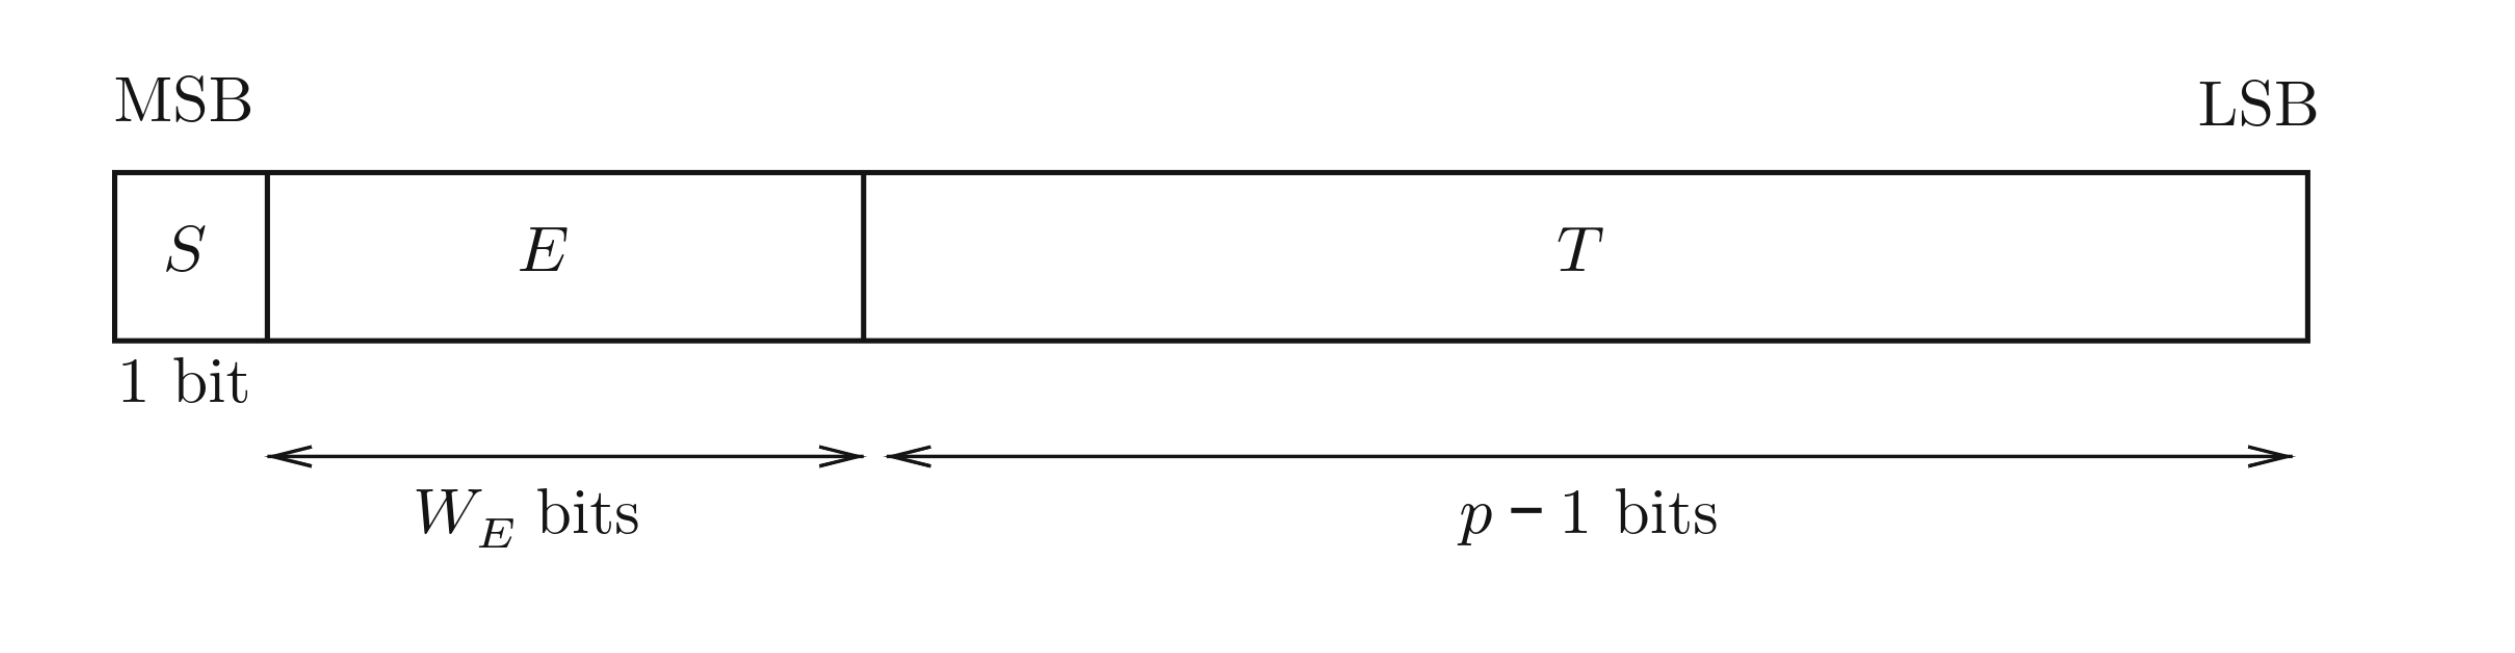
\includegraphics[width=\textwidth]{ieee754_binary_encoding.png}
	\caption{Encoding for the IEEE~754 binary floating-point formats}
	\label{fig:IEEE754-binary-encoding}
\end{figure}
						
\begin{table}[!b]
	\centering
	\begin{tabular}{|l|c|c|}
		\hline
		Biased exponent $N_{e}$ &   
		% start 2nd col title
		\begin{tabular} 
		[c]{@{}c@{}}Trailing \\
		significand \\
		$t_{1}t_{2}\cdots t_{p-1}$
	\end{tabular} &
	% end 2nd col title
	Value represented \\ \hline
	$111\cdots1_{2}$      & $\ne 000\cdots 0_{2}$    & NaN                                                          \\ \hline
	$111\cdots1_{2}$      & $\quad 000\cdots 0_{2}$  & $(-1)^{s}\times\inf$                                         \\ \hline
	$000\cdots0_{2}$      & $\quad 000\cdots 0_{2}$  & $(-1)^{s}\times 0$                                           \\ \hline
	$000\cdots0_{2}$      & $\ne 000\cdots 0_{2}$    & $(-1)^{s}\times 0.t_{1}t_{2}\cdots t_{p-1}\times2^{e_{min}}$ \\ \hline
	$0<N_{e}<2^{W_{E}}-1$ & any                      & $(-1)^{s}\times 1.t_{1}t_{2}\cdots t_{p-1}\times2^{N_{e}-b}$ \\ \hline
	\end{tabular}
	\caption{Encoding to represent special values in the binary formats defined by IEEE~754-2008}
	\label{table:IEEE754-binary-encoding}
\end{table}
						
Representing the set of real numbers in a finite space is impossible; instead, it requires an approximation.
\HL{
	The IEEE~754 format requires the following arithmetic functions tobe correctly rounded:
	addition, subtraction, multiplication, division, and fused multiply-add (FMA).
	Moreover, the square root function and conversion between supported formats must be correctly rounded.
}
Additionally, the standard recommends a list of functions to be correctly rounded~\cite{ieee754_2008-ev}.
There are three directed rounding attributes:
\begin{itemize}
	\item \textit{roundTowardPositive} $RD(x)$ rounds to the largest floating-point less than or equal to $x$.
	\item \textit{roundTowardNegative} $RU(x)$ rounds to the smallest floating-point greater than or equal to $x$.
	\item \textit{roundTowardZero} $RZ(x)$ rounds using $RD(x)$ if $x \ge 0$ or $RU(X)$ if $x \le 0$.
\end{itemize}
There are also two attributes for rounding to the nearest when a floating-point is strictly between two exact representations:
\begin{itemize}
	\item \textit{roundTiesToEven} $RN_{even}(x)$ rounds to the exact representation whose least significant bit is even.
	\item \textit{roundTiesToAway} $RN_{away}(x)$ rounds to the exact representation whose magnitude is the largest.
\end{itemize}
The IEEE~754 standard for the binary formats requires the implementation of all three directed rounding attributes and \textit{roundTiesToEven}.
						
While not a basic format, binary16 is starting to receive more attention and support as it is increasingly being used for computing applications.
For example, it was found that some convolutional neural networks (CNN) perform well with binary16; and even with only 8 bits \HL{{\cite{Muller2018-zm}}}.
Moreover, while most GPUs support only binary32 and binary64, more recent GPU architectures also support the binary16 format.
